\documentclass[a4paper,11pt,oneside]{article}

\usepackage[utf8]{inputenc}
\usepackage[T1]{fontenc}
\usepackage[english]{babel}
\usepackage{amssymb}
\usepackage{amsmath}
\usepackage{graphicx}
\usepackage{float}
\usepackage{hyperref}
\usepackage[dvipsnames]{xcolor}
\usepackage{listings}
\usepackage[top=2cm, bottom=2.5cm, right=2.5cm, left=2.5cm]{geometry}

\renewcommand{\familydefault}{\sfdefault}
\parindent0pt
\parskip6pt
\hypersetup{colorlinks=true,urlcolor=blue,linkcolor=blue}
\lstset{basicstyle=\ttfamily\small, mathescape, literate={Ö}{{\"O}}1 {Ä}{{\"A}}1 {Ü}{{\"U}}1 {ß}{{\ss}}1 {ü}{{\"u}}1 {ä}{{\"a}}1 {ö}{{\"o}}1}

\begin{document}

\title{Short summary:\\Methods of statistical quality control}
\author{Alexander Herzog\\\href{mailto:alexander.herzog@tu-clausthal.de}{\small\texttt{alexander.herzog@tu-clausthal.de}}}
\date{}

\maketitle

Statistical quality control is used both to monitor ongoing processes and to inspect incoming goods. While the aim of process monitoring is to continuously check that the parameters of a (manufacturing) process are within the respective target ranges, statistical monitoring of incoming goods is about ensuring the quality of delivered workpieces without having to carry out a \emph{full inspection}. Full inspections are often either not possible because the workpiece to be inspected is destroyed during the inspection, or a full inspection would not make economic sense:

\begin{itemize}
\item
Batches of New Year's Eve rockets delivered cannot be subjected to a full inspection before sale.
\item
For large deliveries of screws, washers, and similar small parts in a production facility, a full inspection would be possible, but not economical considering the value of the individual components.
\end{itemize}



\section{Sample inspection}

Instead of a full inspection, only a random sample (of size $n\in\mathbb N$) of the delivery (of size $N\in\mathbb N$, where $N$ is significantly larger than $n$) is checked in these cases. The following considerations are based on the assumption that a \emph{good-bad test} is possible, i.\,e., that it can be clearly determined whether a workpiece meets the defined requirements or not. It is therefore a yes/no distinction. In a full inspection, the supplier and customer would set a clear quality limit for deliveries -- e.\,g., $p=0.1\%$. If, out of $N=10,000$ screws delivered, no more than $N\cdot p=10,000\cdot0.1\%=10$ are defective, the delivery is accepted. Otherwise, it is returned to the supplier. With random sampling, such absolute statements are no longer possible.



\section{Good and bad limits}

Therefore, the supplier and customer agree on an Acceptance Quality Limit (AQL, good limit) and a Limiting Quality (LQ, bad limit). Deliveries that meet the acceptance limit should ``almost always'' be accepted. Deliveries that violate the limiting quality limit in terms of the proportion of rejected parts should ``almost never'' be accepted. If the acceptance quality and limiting quality limits are moved closer and closer together, the sampling plan increasingly approaches a full inspection.

\subsection*{Terms for good and bad limits}

\begin{eqnarray*}
p_{1-\alpha}&:=&\text{Acceptance Quality Limit; Good limit; Defect rate when deliveries}\\
~&~&\text{are almost always to be accepted}\\[2ex]
1-\alpha&:=&\text{Requested minimum acceptance probability for deliveries}\\
~&~&\text{with a defect proportion of no more than}~ p_{1-\alpha}\\[2ex]
p_\beta&:=&\text{Limiting Quality; Bad limit; Defect rate when deliveries}\\
~&~&\text{are almost always to be rejected}\\[2ex]
\beta&:=&\text{Requested maximum acceptance probability for deliveries}\\
~&~&\text{with a defect proportion of}~ p_{\beta} ~\text{or more}
\end{eqnarray*}

\begin{figure}[H]
\begin{center}
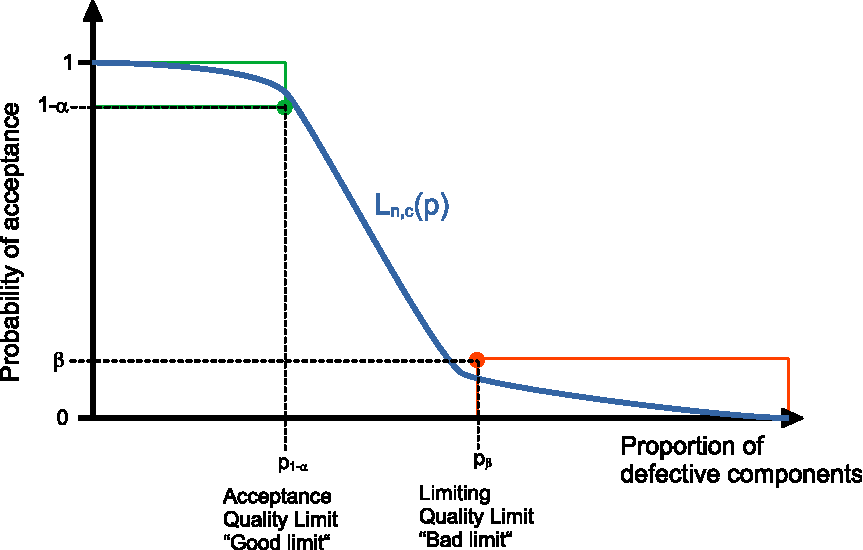
\includegraphics[width=0.7\textwidth]{OperationCharacteristics_en.pdf}
\end{center}
\caption{Acceptance probability, good and bad limits for a sample inspection}
\label{fig:L}
\end{figure}



\section{Errors of the 1st and 2nd type}

The aim of defining good and bad limits and the associated acceptance probabilities at these two quality points is to accept ``good'' deliveries whenever possible and reject ``bad'' deliveries whenever possible.

If the sample test indicates that the delivery is good and it actually is, or if the sample test indicates that the delivery is bad and it actually is, then the test has worked. If the sample test result and the reality do not match in relation to the entire delivery, then the test has made a mistake:

\begin{itemize}
\item
If a delivery is rejected on the basis of an unsuccessful sample test, even though it would have met the quality targets in relation to its overall quantity, this is referred to as a \emph{Type 1 error} (supplier risk).
\item
If a delivery is accepted on the basis of good sampling results, even though it does not meet the quality objectives in relation to its overall quantity, this is referred to as a \emph{Type 2 error} (customer risk).
\end{itemize}

The supplier would like to minimize type 1 errors (his delivery is rejected even though it is good). The customer would like to minimize type 2 errors (delivery is accepted even though it is bad). The probabilities of these errors can be controlled by choosing $p_{1-\alpha}$, $1-\alpha$, $p_\beta$ and $\beta$. The smaller the error probabilities that the sample test is to deliver, the more delivered workpieces have to be checked in each case, i.\,e.\ the more the sample test has to approach a full inspection.

When determining the good and bad limits, it is therefore always necessary to weigh up the required quality of the test against the testing effort involved.



\section[n-c Sample plans]{$n$-$c$ Sample plans}

Based on these preliminary considerations, the following general procedure for setting up and applying a sampling plan results:

\begin{enumerate}
\item
The supplier and customer jointly agree on the quality criteria to be met. This can be, for example, the joint determination of the good limit ($p_{1-\alpha}$ and $1-\alpha$) and the bad limit ($p_\beta$ and $\beta$).
\item
An algorithm is applied to calculate a sampling plan that ensures that the required criteria are met. Such a plan then stipulates that $n\in\mathbb N$ parts must be inspected from deliveries of size $N\in\mathbb N$. If there are more than $c\in\mathbb N_0$ defective parts among these $n$ parts, the delivery is rejected (otherwise it is accepted).
\item
A random sample of $n$ parts is taken from each incoming delivery. These are inspected. If the sample contains more than $c$ defective parts, the delivery is either rejected immediately or (if reasonably possible) a full inspection is carried out.
\end{enumerate}



\section{Operation characteristics}

From a stochastic perspective, taking and testing a sample from a population is a \emph{urn model}:

\begin{itemize}
\item
An urn contains $N\in\mathbb N$ balls (total size of the delivery).
\item
$n\in\mathbb N$ balls are taken from the urn without replacement, where $n\le N$ (sample size).
\item
The number of red balls (defective workpieces) is $R\in\mathbb N_0$, where obviously $R\le N$. In the case of a delivery, $R$ is unknown.
\item
From $R$ (unknown) and $N$ (known), the proportion of red balls or defective components can then also be determined: $p=\frac{R}{N}$.
\end{itemize}

Urn models in the case of drawing without replacement are described by the \emph{hypergeometric distribution}. According to this, the probability of drawing exactly $k\in\mathbb N_0$, $k=0,\ldots,n$, red balls or defective components, or having them in the sample, is:
$$
P(X=k)=
\mathrm{Hg}_{N,R,n}(k)=
\frac{\binom{R}{k}\binom{N-R}{n-k}}{\binom{N}{n}}.
$$
The probability that a sample of size $n$ from a shipment of $N$ parts (including $R$ defective parts) contains at most $c\in\mathbb N_0$ defective parts is therefore:
$$
P(X\le c)=
\sum_{k=0}^c \mathrm{Hg}_{N,R,n}(k)=
\sum_{k=0}^c \frac{\binom{R}{k}\binom{N-R}{n-k}}{\binom{N}{n}}.
$$
With the approximation $p\approx\frac{R}{N}$ respectively $R:=\lfloor N\cdot p\rfloor$, one refers to
$$
L_{n,c}(p):=
P(X\le c)=
\sum_{k=0}^c \frac{\binom{\lfloor N\cdot p\rfloor}{k}\binom{N-\lfloor N\cdot p\rfloor}{n-k}}{\binom{N}{n}}
$$
as the \emph{operation characteristics} of the $n$-$c$ sample plan (also see figure \ref{fig:L}).



\section[Construction of n-c sample plans]{Construction of $n$-$c$ sample plans}

The goal now is to find an operation characteristic $L_{n,c}(p)$ (or, more precisely, parameters $n$ and $c$) such that
\begin{enumerate}
\item
the operating characteristic meets the condition at the good limit:\\
$L_{n,c}(p_{1-\alpha})\ge1-\alpha$,
\item
the condition at the bad limit is met: $L_{n,c}(p_\beta)\le\beta$ and
\item
the testing effort is minimal: $n\to\mathrm{Min}$.
\end{enumerate}

\subsection{Günther's algorithm}

In general, the more parts $n$ are inspected, the less likely it is that a shipment will be accepted (given a fixed maximum number of allowed defective parts $c$ in the sample). At the same time, the more defective parts $c$ are allowed (given a constant sample size $n$), the more likely it is that a shipment will be accepted. It follows that:

\begin{itemize}
\item
If the operating characteristic does not meet the acceptance limit (good deliveries are rejected with too high a probability), $c$ is increased (and the operating characteristic is thus shifted upwards).
\item
If the operating characteristic does not meet the limiting quality criterion (bad deliveries are accepted with too high a probability), $n$ is increased (thereby shifting the operating characteristic downward).
\end{itemize}

This approach is systematically summarized in Günther's algorithm:

\begin{enumerate}
\item
\emph{Initialization ($n:=1$, $c:=0$):}~\\
We start with a sample size of $n:=1$, in which no defective components may be present for the entire delivery to be accepted ($c:=0$).
\item
\emph{Check whether the plan meets the conditions ({\color{ForestGreen}$L_{n,c}(p_{1-\alpha})\ge1-\alpha$} $\wedge$ {\color{ForestGreen}$L_{n,c}(p_\beta)\le\beta$} ?):}~\\
If this sampling plan meets both the good and bad limits, the process is complete and an optimal sampling plan (i.\,e., a sampling plan with a minimum sample size) has been found.
\item
\emph{{\color{Red}$L_{n,c}(p_\beta)>\beta$} $\to$ $n:=n+1$:}~\\
If the sampling plan does not yet meet the bad limit (poor deliveries are accepted with too high a probability), $n$ is increased. This step is then repeated.
\item
\emph{{\color{Red}$L_{n,c}(p_{1-\alpha})<1-\alpha$} $\to$ $c:=c+1$, $n:=c$:}~\\
If the plan (as determined by step 3) now meets the bad limit but not yet the good limit, $c$ is increased by one, $n$ is set to the smallest possible meaningful value ($c$), and the process continues with step 3.
\item
\emph{End ({\color{ForestGreen}$L_{n,c}(p_{1-\alpha})\ge1-\alpha$} $\wedge$ {\color{ForestGreen}$L_{n,c}(p_\beta)\le\beta$}):}~\\
The two previous steps ensure that the plan complies with both the upper and lower limits.
\end{enumerate}

In pseudocode, Günther's algorithm can be formulated as follows:

\begin{lstlisting}[inputencoding={utf8},frame=single]
// Initialization
n:=1
c:=0

// Already finished?
if ($L_{n,c}(p_{1-\alpha})\ge1-\alpha$ && $L_{n,c}(p_\beta)\le\beta$) $\to$ Ende

// Outer loop: increasing c
while (true) {
  // Inner loop: increasing n until the bad limit is maintained
  while ($L_{n,c}(p_\beta)>\beta$) {
    n++
  }
  // Good limit also maintained?
  if ($L_{n,c}(p_{1-\alpha})\ge1-\alpha$) $\to$ Ende

  // Else: increase c and next round in outer loop
  c++
  n:=c
}
\end{lstlisting}

\subsection[Chi-square method]{$\chi^2$ method}

To determine an optimal sampling plan based on Günther's algorithm, two nested loops have to be executed. In each step of the inner loop, $L_{n,c}(p)$ has to be calculated, which in turn is a sum over a fraction of three binomial coefficients. To calculate a binomial coefficient, a product over a whole series of factors has to be calculated. This gives the algorithm a total complexity of $O(n^4)$. If the calculation is performed by computer, this complexity is not a problem. However, if the calculation is performed with pen and paper, the effort involved would be considerable. Therefore, when the need for sampling inspection arose with the advent of industrial mass production, an (approximate) method with lower complexity was sought.

The $\chi^2$ method provides exactly this: If the delivery quantity $N$ is large and the expected proportion of defective components $p$ is small, then instead of sampling without replacement (hypergeometric distribution), we can switch to the Poisson distribution:

$$
P(X=k)=\frac{\lambda^k}{k!}\exp(-\lambda),
$$
where $\lambda:=n\cdot p$. Next we have:

\begin{equation}\label{eq:LPoisson}
P(X\le c)=
\sum_{k=0}^c \frac{\lambda^k}{k!}\exp(-\lambda)=
1-G(2\lambda,2(c+1)),
\end{equation}
where $G$ is the $\chi^2$ distribution with $2(c+1)$ degrees of freedom.

Assuming that for the operation characteristic $L_{n,c}(p):=1-G(2np,2(c+1))$ holds, the conditions for the good and bad limits ($L_{n,c})(p_{1-\alpha})\ge1-\alpha$ and $L_{n,c}(p_\beta)\le\beta$) can be rewritten as follows:

\begin{align*}
L_{n,c}(p_{1-\alpha}) \ge 1-\alpha
&\iff 1-G(2np_{1-\alpha},2(c+1))\ge1-\alpha\\
&\iff G(2np_{1-\alpha},2(c+1)) \le\alpha\\
&\iff G^{-1}(\alpha,2(c+1))\ge2np_{1-\alpha}\\
&\iff \frac{G^{-1}(\alpha,2(c+1))}{2p_{1-\alpha}}\ge n,\\[2ex]
L_{n,c}(p_\beta)\le\beta
&\iff 1-G(2np_\beta,2(c+1))\le\beta\\
&\iff G(2np_\beta,2(c+1))\ge1-\beta\\
&\iff G^{-1}(1-\beta,2(c+1))\le2np_\beta\\
&\iff \frac{G^{-1}(1-\beta,2(c+1))}{2p_\beta}\le n
\end{align*}

The algorithm for determining $n$ and $c$ can then be reduced to an iteration over $c$. In each iteration step, two values of the inverse of the $\chi^2$ distribution have to be calculated. These values are usually available in tabular form (for working with pen and paper), so that no calculations are necessary here; instead, only two values need to be read from a table. This results in the following calculation rule:

Let $G(x,k)$ be the distribution function of the $\chi^2$ distribution in $k\in\mathbb N$ degrees of freedom at the point $x\ge0$. Then $c$ is increased until both of the following inequalities are satisfied:

$$
\frac{G^{-1}(1-\beta;2(c+1))}{2p_\beta}\le n\le\frac{G^{-1}(\alpha;2(c+1))}{2p_{1-\alpha}}.
$$

When evaluating by computer, the effort required to calculate $G^{-1}$ is usually more significant than the 4 nested loops (each of which usually only has small values).

\subsection{Philips sample plan}

The method developed by Philips for determining sampling plans represents a generally different option instead of specifying a good and a bad limit. The so-called \emph{indifference point} is considered for this purpose. This is the proportion of defective items in a delivery at which the delivery is accepted according to the sampling plan with a probability of exactly 50\,\%:

$$
L_{n,c}(p_{0{,}5})=50\,\%.
$$

At this point $p_{0.5}$, the \emph{steepness} of the operating characteristic is now specified. The steepness $h_0$ does not simply refer to the derivative of $L(p)$ at the point $p=p_{0.5}$, but rather to the following expression:

$$
h_0:=
\left.-\frac{p}{L_{n,c}(p)}\cdot\frac{\mathrm{d}L_{n,c}(p)}{\mathrm{d}p}\right|_{p:=p_{0{,}5}}=
-\frac{p_{0{,}5}}{0{,}5}\cdot L'_{n,c}(0{,}5)=
-2p_{0{,}5}\cdot L'_{n,c}(0{,}5).
$$

If (as in the $\chi^2$ method) the Poisson distribution is again assumed as the model distribution for the operating characteristic (see \eqref{eq:LPoisson}), the result is:
$$
h_0:=
-2p_{0{,}5}\cdot
\left(-\frac{(np_{0{,}5})^{c+1}}{p_{0{,}5}c!}\exp(-np_{0{,}5})\right)=
\frac{2(np_{0{,}5})^{c+1}}{c!}\exp(-np_{0{,}5}).
$$

Using the same transformations as in the $\chi^2$ method, it can be shown that:
$$
L_{n,c}(p_{0{,}5})=0{,}5 ~\iff~ \frac{G^{-1}(0{,}5,2(c+1))}{2p_{0{,}5}}=n.
$$

Instead of having to specify two points (good limit and bad limit) for the operating characteristic, only the proportion of rejected parts that is still acceptable in exactly 50\% of cases and the degree of selectivity required for the test at this point are specified: The greater the steepness of the sampling plan at the indifference point, the better it distinguishes between good and bad deliveries (but of course, the higher the testing effort).

To determine the values $n$ and $c$ that satisfy the required steepness (as jointly specified by the supplier and customer), $c$ is iterated:

\begin{enumerate}
\item
We iterate over $c$ starting with $c=0$.
\item
In each step, the value $n$ associated with $c$ is first determined using the inverse of the $\chi^2$ distribution:
$$
n:=\left\lceil\frac{G^{-1}(0{,}5;2(c+1))}{2p_{0{,}5}}\right\rceil.
$$
\item
Then we check whether the condition on $h_0$ is satisfied:
$$\frac{2(np_{0{,}5})^{c+1}}{c!}\exp(-np_{0{,}5})\ge h_0.$$
If this is the case, a minimal sampling plan that meets the requirements has been found. Otherwise, $c$ is increased by one and the process continues with step 2.
\end{enumerate}



\section{Average slip-through and maximum average slip-through}

For the following considerations, it is assumed that deliveries that do not meet the quality standards of the $n$-$c$ sampling plan are not returned to the supplier, but instead undergo a full inspection in order to identify all defective parts. If a delivery of size $N$ actually contains $R$ defective parts, the following applies to the number of defective parts found:

\begin{itemize}
\item
At most $c$ defective parts in the sample:\\
Number of defective parts found: $c$
\item
More than $c$ defective parts in the sample:\\
Number of defective parts found: $R$
\end{itemize}

If we move from the absolute number of not found defective parts, which depends on the delivery size, to the relative proportion of defective parts not found, we arrive at the \emph {Average slip-through} (Average outgoing quality, AOQ). This indicates the statistical proportion of defective parts or the probability of encountering a defective workpiece in production after the initial statistical quality test. According to the above considerations, the following applies to the average outgoing quality $\mathbf{E}[Y]$:
$$
\mathbf{E}[Y_p]=
p\cdot P(X\le c) + 0\cdot P(X>c)=
p\cdot L_{n,c}(p).
$$

If $p$ is very low, only a few deliveries are subjected to a full inspection, but only a few defective components enter production because there are only a few defective components overall. If $p$ is very high, many deliveries do not meet the quality specifications and are therefore subjected to a full inspection, which weeds out all defective components. In this case, too, only a few defective components enter production. Consequently, the maximum is achieved with medium defect rates. The maximum number of defective components in production that have to be expected (when $p$ is unknown) is the \emph{maximum average slip-through} (Average outgoing quality limit, AOQL):
$$
\mathrm{AOQL}:=
\max_{0\le p\le1} \mathbf{E}[Y_p].
$$



\section{Average testing effort}

Analogous to the considerations regarding the mean slip-through, the mean testing effort $\mathbf{E}[M]$ can also be determined. When using an $n$-$c$ sampling plan, a sample of size $n$ is tested in each case. If the delivery is accepted, the mean inspection effort is $n$. If the delivery is rejected, a full inspection of all $N$ parts is performed. This results in the number of parts to be inspected $M$:
$$
M=
\begin{cases}
n, & ~\text{if}~ X\le c\\
N, & ~\text{if}~ X>c.
\end{cases}
$$
For the average testing effort $\mathbf{E}[M]$, the following applies:
$$
\mathbf{E}[M]=
n\cdot P(X\le c) + N\cdot P(X>c)=
n\cdot L_{n,c}(p) + N\cdot(1-L_{n,c}(p)).
$$



\begin{thebibliography}{9}

\bibitem{Banks89}
J.~Banks:
\emph{Principles of Quality Control},
John Wiley and Sons, New York, 1989.

\bibitem{Montgomery91}
D.\,C.~Montgomery:
\emph{Introduction to Statistical Quality Control},
8nd edition, John Wiley and Sons, New York, 2020.

\bibitem{RinneMittag95}
H.~Rinne und H.–J.~Mittag:
\emph{Statistische Methoden der Qualitätssicherung},
3.~Auflage, Carl Hanser Verlag, München, 1995.

\bibitem{Uhlmann82}
W.~Uhlmann:
\emph{Statistische Qualitätskontrolle},
7.~Auflage, Springer–Verlag, Stuttgart, 2013.

\end{thebibliography}

\end{document}
